\section{Video Streaming Applications}

Efficiently delivering streaming video over the internet has long been an active research topic. Non-linearity, rich user interactions and diversification of media sources have driven users from consuming terrestrial television or hard copy video to internet based media platforms.
These platforms and their underlying technologies can be categorised by (1) offered media types and (2) content distribution architecture. Some platforms offer pre-produced videos, be it professional movies or amateur vlogs, to be streamed on demand (\gls{vod}). Other platforms offer live video streams with realtime viewer interactions.
Both type of video offerings can be found to be built upon a centralised or decentralised streaming architecture. \vref{fig:media-platforms-quadrant} shows examples of platforms arranged by category.

\begin{figure}
\centering
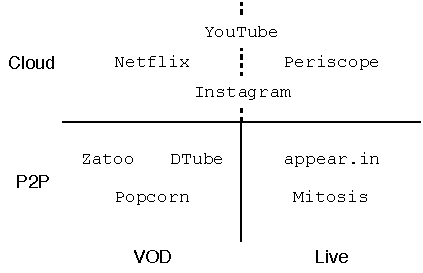
\includegraphics[width=.75\textwidth]{graphics/media-platforms-quadrant.pdf}
\caption{Examples of media platforms by delivery and content category}
\label{fig:media-platforms-quadrant}
\end{figure}

\subsection{Centralised Streaming}

The most popular video platforms, YouTube\footnote{Youtube. URL: {https://www.youtube.com}} and Netflix\footnote{Netflix. URL: {https://www.netflix.com}}, currently account for TODO percent of internet traffic \cite[p 18]{phenomena-report}. Dealing with such extreme user numbers, centralised video delivery architectures are complex and costly \cite{market-driven-p2p}. To deliver compelling \gls{qos} to users, platforms must ensure their networks can retrieve content from a live source or their catalogue with low latency and deliver it in a format optimal for the end users' device and network capabilities. There must be a global server infrastructure for storing, caching and delivering content. Platforms that allow user-generated content must also provide ingress servers, that accept video uploads from users.

These expenses drive platform providers to heavy use of video advertising or subscription models.

\paragraph{Ingress}
Platforms with user-generated content have grown in popularity and significance and, according to \citet{twitch-case}, can be characterised by opening content creation to all of their users and allowing video consumers to give realtime feedback in the form of chats or likes. This interactivity poses tight constraints on latency, or users can become frustrated \cite{TODO}. Periscope, for example, constraints its chat function to the first 100-200 viewers per stream \cite{TODO}. These early participants will be provided with a low latency \gls{rtmp} video stream \cite{TODO}. Subsequent viewers will be served an \gls{hls} video from a global \gls{cdn}. The latter introduces two further sources of delay \cite[\S2-3{periscope-experience}: 1) \gls{hls} segments the video into smaller files, so the duration of such a chunk adds to overall latency. 2) According to network analysis by \citet{periscope-experience} Periscope uses different \textit{Cloud Computing} providers for ingress and \gls{cdn} use.

Twitch, for example, reserves computationally expensive trans-coding of live streams for its premium users \cite[\S2]{twitch-study}. That means, viewers of free channels can only receive the video in the format it was originally uploaded in. Since, unlike Periscope, Twitch also offers access to streams through their website \cite{TODO}, this excludes users from content in formats incompatible with their browser. If a channel subscribes to their premium service trans-coding introduces a delay of up to 10 seconds \cite[\S4.2]{twitch-study}.

\citet[III A.]{content-harvest-network} argue, that the so-called \textit{first mile} between the live video producer and the systems ingress server bears a significant optimisation opportunity. Because upload may be hindered by unstable network conditions, any delay directly impacts the \gls{qoe} of all viewers of the stream.

\paragraph{Transcoding}
SFU or whatevs, Transcoding units

\paragraph{Quality of Experience}
\citet*{personalized-live-streaming-experience} propose schemes to optimise variable video bitrates to improve the perceived \gls{goe} for viewers.

\paragraph{Delivery}
Because HTTP streaming protocols are not built for multicasting, even popular live streams, that many users view simultaneously, have to be delivered to each device individually. Therefore, providers use multiple server farms \cite{TODO-network-book} in strategic geographic locations of their user market. Streams must be routed intelligently from ingress to egress locations within a provider's network. Predicting a streams popularity and allocating resources in locations geographically close to viewer demand can help reduce latency \cite{TODO}.

According to \citet{TODO}, the strategy of Twitch is to serve content from the vicinity of every \gls{ipx}. Social photo and video sharing site Instagram, on the other hand, goes even further and serves content from locations in most major cities of its user market \cite{TODO}. These efforts to bringing server resources as close to users as possible are often referred to as edge or fog computing \cite{fog-computing, object-store-fog-edge-ipfs}.

Despite all efforts, especially less financially secured platforms struggle to come up with enough resources to deliver \gls{qos} without compromise.
...

- Cisco says mobile video streaming is lit

\paragraph{Social Aspects}
censorship vs piracy

\begin{figure}
\centering
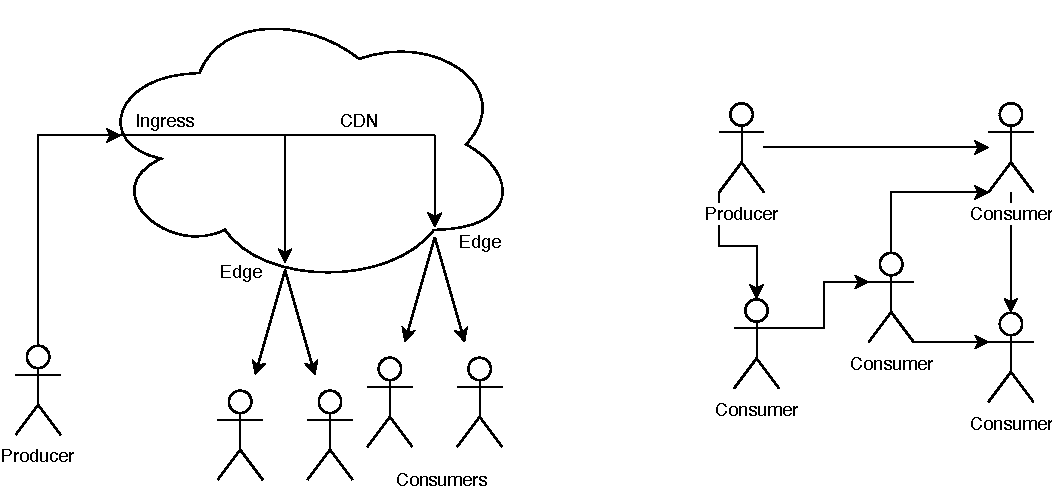
\includegraphics[width=.5\textwidth]{graphics/streaming-types.pdf}
\caption{Centralised versus decentralised video streaming architecture}
\label{fig:pipeline}
\end{figure}

\subsection{Decentralised Streaming}

In contrast, decentralised video streaming technologies build multicast streaming on top of an overlay network in the application space. These overlays can be categorised as tree or mesh shaped or a combination thereof. Each peer becomes part of the network and has to assist in its maintenance and content delivery. Decentralised streaming approaches need to handle peers joining and leaving the network, called \textit{peer churn} \cite[\S7.5]{tanenbaum_wetherall_2011}. Like centralised platforms, they must also cope with varying network performance of its users. However, upload capacity becomes a important factor for every peer, not just content producing ones. This means, that finding a compromise between the depth of the tree or mesh structure and the amount of outward connections each node has to maintain is crucial for the system's performance \cite[\SIII.A]{multicast-problems}.

\paragraph{Content Discovery}
In fully decentralised approaches, content discovery is another issue to consider. Whereas centralised media platforms can index, aggregate and even recommend content to users by consulting their databases, decentralised applications lack such central look–up tables by design. Information about peer and content availability must be propagated through the network, creating further traffic and computational overhead.

\paragraph{DONet}
DONet, which was first implemented in the widely researched CoolStreaming, was introduced by \citet{coolstreaming}. It constructs a mesh of peers gossiping (\ref{gossiping}) about available content, members of the network and direct connections. Each peer maintains an incomplete view of the network and a set of peer partnerships. Video streams are split into segments of a defined length and the segments are broadcasted through the network individually. Nodes request segments from their partners, cache segments they receive and add them to their own playback buffer \cite[\SIII.B]{coolstreaming}. When a node detects a stalling upstream partner, it tries to find a better source \cite[\SIV.A]{coolstreaming-design-theory}.

\paragraph{AnySee}
Mesh–based streaming networks like CoolStreaming can achieve good utilisation of peer bandwidth and discover fresh peers with low overhead \cite[\SII]{anysee}. However, \citet[\SIII]{anysee} find that, "Due to the random selection algorithm, the quality of service cannot be guaranteed, such as the startup delay". AnySee evolves \gls{p2p} streaming nodes with a set of manager components \citep[\SIII.B-F]{anysee}. 1) The \textit{Mesh-based Overlay Manager} actively tries to align the mesh network with the physical network by flooding its neighbourhood with \gls{ttl}–bound messages and re–aligning overlay connections. 2) The \textit{Single Overlay Manager} measures and propagates a nodes time offset from the video source and ensures the streaming path is arranged according to this offset. 3) The \textit{Inter-overlay Optimization Manager} secures a set of backup streaming paths through a delay–based tracing algorithm. 4) The \textit{Key Node Manager} queues requests and prioritises stream requests from other peers. 5) The \textit{Buffer Manager}'s task is to request upstream video and providing it to the applications \gls{ui}.

+ continuouity index
+ buffer size 120 vs 40 seconds
- timestamps be shitty

Further, AnySee introduces location awareness to encourage peer partnering close to their geographical vicinity \citep[\SV.B.1]{anysee}. In their initial implementation, this was achieved by matching \gls{ip} addresses of their research network (\gls{cernet}) to known building locations.

\paragraph{HLPSP}
Another refinement to CoolStreaming was introduced by \citet*{hlpsp} called \gls{hlpsp}. This approach creates a layered hierarchy in which peers with higher uploads are positioned in levels closer to the video source. Peers then serve other peers in their own or subsequent levels \cite[\S3]{hlpsp}. The gauging of bandwidth is left up to the network entry point (also referred to as signal server or tracker). This central server assigns a level to a newcomer and provides a list of possible connection partners. If not enough suitable partners are found, the tracker scans the hierarchy and downgrades peers to free capacity on the newcomers level \cite[\S3.3.2]{hlpsp}. This results in efficient bandwidth utilisation, but only accounts for single source scenarios.

- routing
- overlay creation -> timetofirstbyte
- ...problems of streamer cite
